\section{Documentation}
\vspace{1cm}

Afin de faciliter la reprise de cette partie par mon tuteur et mes successeurs, j’ai également écrit et mis en ligne une documentation complète. Celle-ci est écrite en Markdown (.md) et joue le rôle d’un cahier des spécifications techniques, permettant ainsi la compréhension du code en profondeur. 

\begin{figure}[!h]
    \centering
    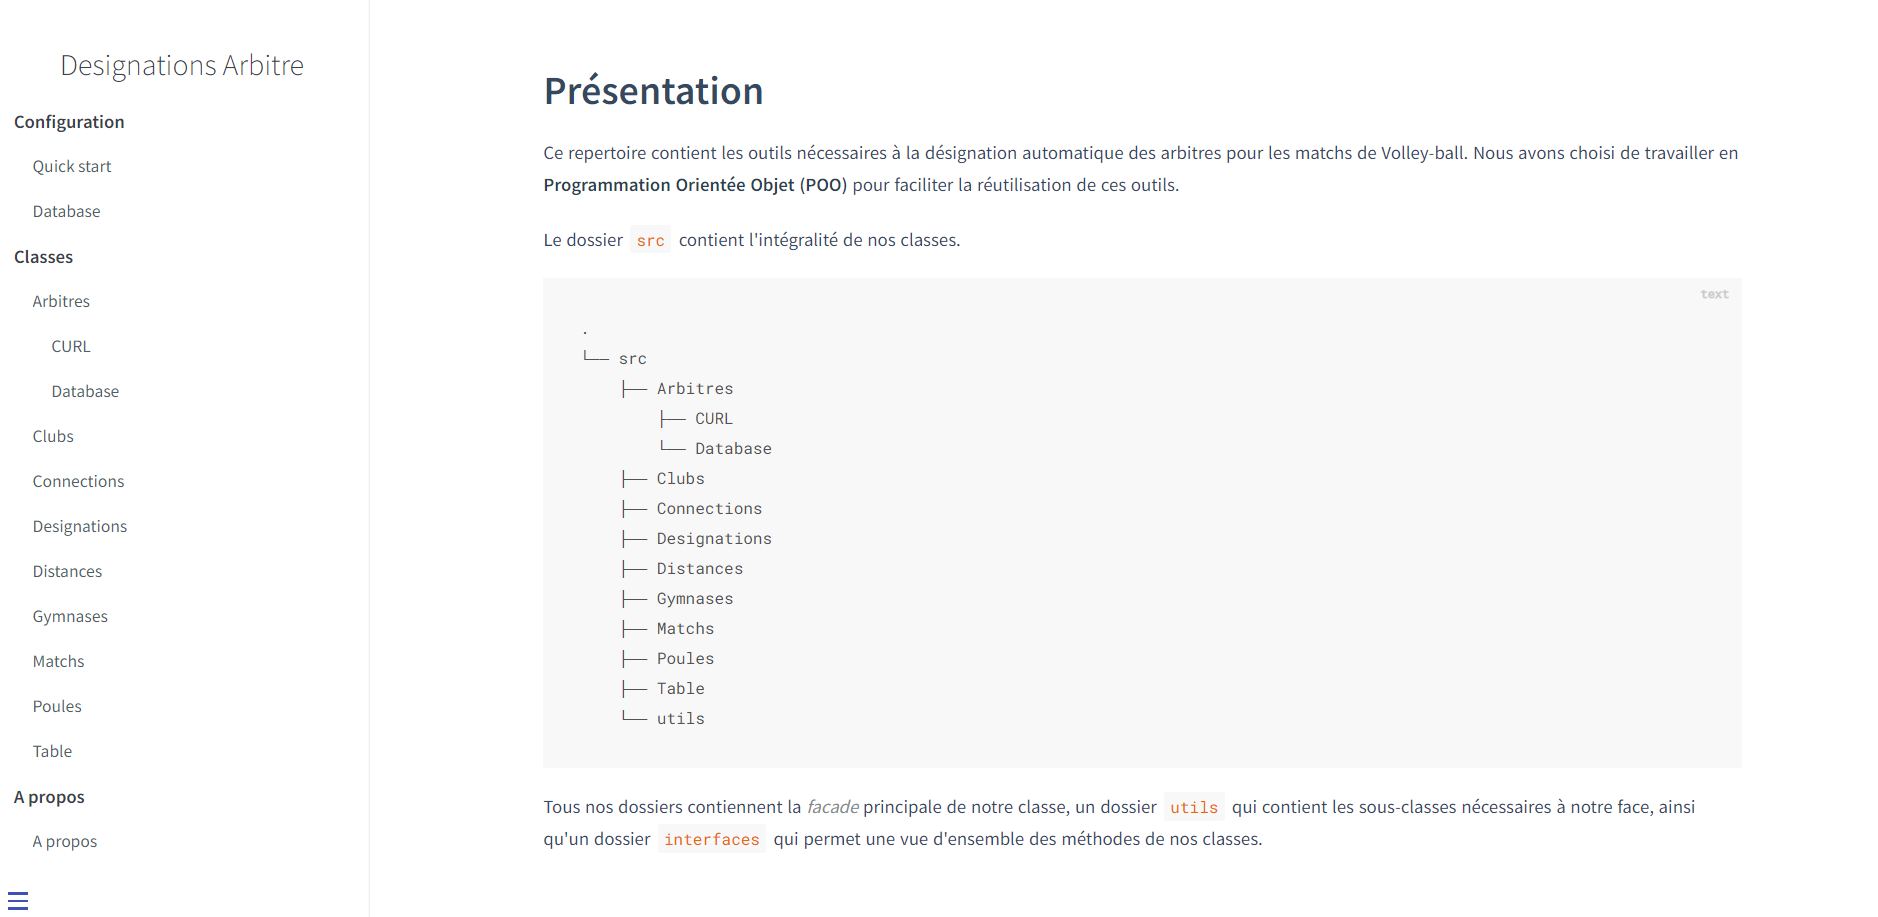
\includegraphics[width=\linewidth]{doc}
    \caption{Documentation en ligne pour le projet}
\end{figure}

La mise en page est gérée par \colored{Docsify}, une bibliothèque Javascript qui permet de convertir les fichiers markdown en pages HTML. Celle-ci permet ainsi de faciliter le rendu de la documentation, ce qui permet de se concentrer sur son contenu.\\

Pour la mise en ligne, j’ai opté pour le service gratuit de Google Firebase afin d’avoir une première intéraction avec cet outil.